\documentclass[11pt]{article}

% Use wide margins, but not quite so wide as fullpage.sty
\marginparwidth 0.5in 
\oddsidemargin 0.25in 
\evensidemargin 0.25in 
\marginparsep 0.25in
\topmargin 0.25in 
\textwidth 6in \textheight 8 in
% That's about enough definitions

% multirow allows you to combine rows in columns
\usepackage{multirow}
% tabularx allows manual tweaking of column width
\usepackage{tabularx}
% longtable does better format for tables that span pages
\usepackage{longtable}
\usepackage{graphicx}
\usepackage{caption}
\usepackage{fixltx2e}
\usepackage{amsmath}
\usepackage{float}
% \usepackage[T1]{fontenc}

\providecommand{\e}[1]{\ensuremath{\times 10^{#1}}}

\begin{document}

% this is an alternate method of creating a title
\hfill\vbox{\hbox{Huang, Jonathan (jhh283)}
      \hbox{Lakin, Neil (nrl39)}
      \hbox{CS5785: Modern Analytics}  
      \hbox{\today}}\par

\bigskip
\centerline{\Large\bf CS5785: Homework 1}\par
\bigskip

\section{Crazy Taxi}
\emph{Pre-Note: Code referenced in this document (without line numbers) should have corresponding comments in the .py file indicating what question the code was for. I chose to not include line numbers because of the constantly changing state of my code and for fear of misleading you guys.}

\begin{enumerate}
  \item[a] The data was successfully downloaded and loaded. The code used to open and pre-process the data can be found in retrieve.py [retrieve\_data function]. For part a, the code calling retrieve.py can be found in main.py.

  \item[b] The distance calculation script was incorporated into util.py [get\_distance function]. This calculation was called from retrieve.py in line 21. The minimum and maximum calculated distances between pickup and dropoff (before and after outlier filtering) can be seen in table 1. The initial outlier filtering method chosen (implemented in outlier.py [main, mean\_remove, and remove\_zeros functions] and called in main.py) is as follows:

  \begin{enumerate}
  \item[1] Remove any data points where trip time is 0 - where trips with time 0 were assumed to be incorrectly recorded
  \item[2] Remove any data points where the calculated distance between pickup and dropoff is greater than 1 standard deviation from the mean 
  \end{enumerate}

  In this case, a cutoff of 1 standard deviation was chosen because it maintained the 26 mile max which makes sense in the context of New York City.

  \begin{center}
    \captionof{table}{b - Calculated Min and Max Distance (mi)} 
    \begin{tabular}{| c | c | c |}
    \hline
    Distance (mi) & Before Filtering & After Filtering \\ \hline
    Min & 0 & 0 \\ \hline
    Max & 5389.36258565 & 26.7882223084 \\ \hline
    \end{tabular}
  \end{center}

  \item[c] The code used to create the scatterplots can be found in plot.py [plot\_data function] which is called from main.py. The figures are included below (Figures 1-3).

  \begin{figure}[p]
  \centering
  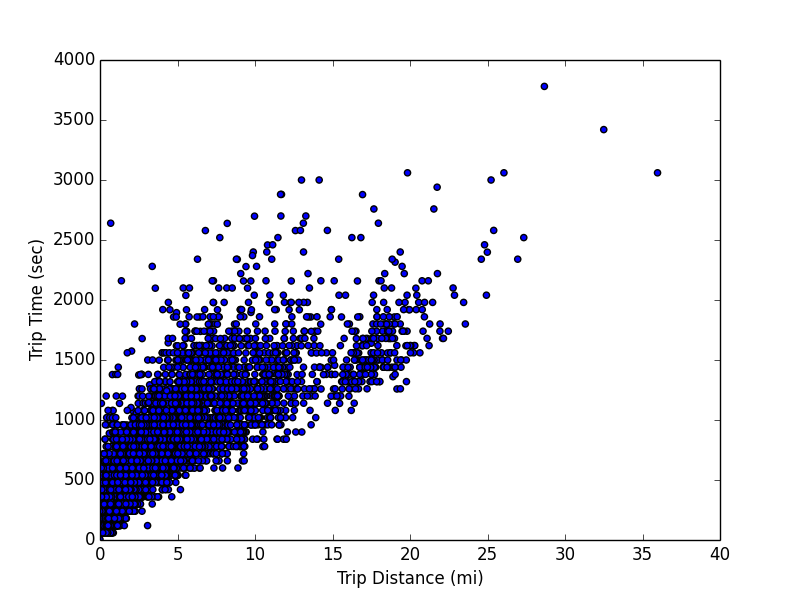
\includegraphics[scale=0.6]{1-mean.png}
  \caption{c - Trip Distance (mi) vs Trip Time (sec)}
  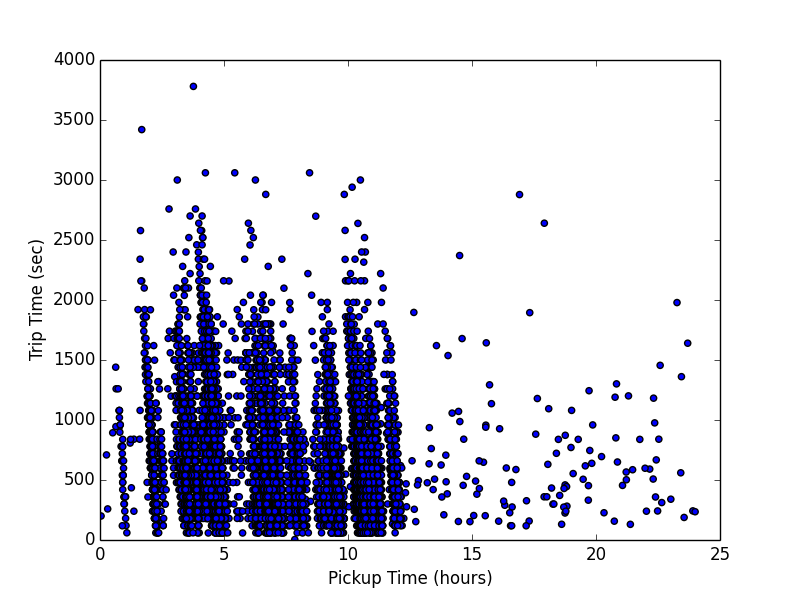
\includegraphics[scale=0.6]{2-mean.png}
  \caption{c - Pickup Time (hrs) vs Trip Time (sec)}
  \end{figure}

  \begin{figure}[ht]
  \centering
  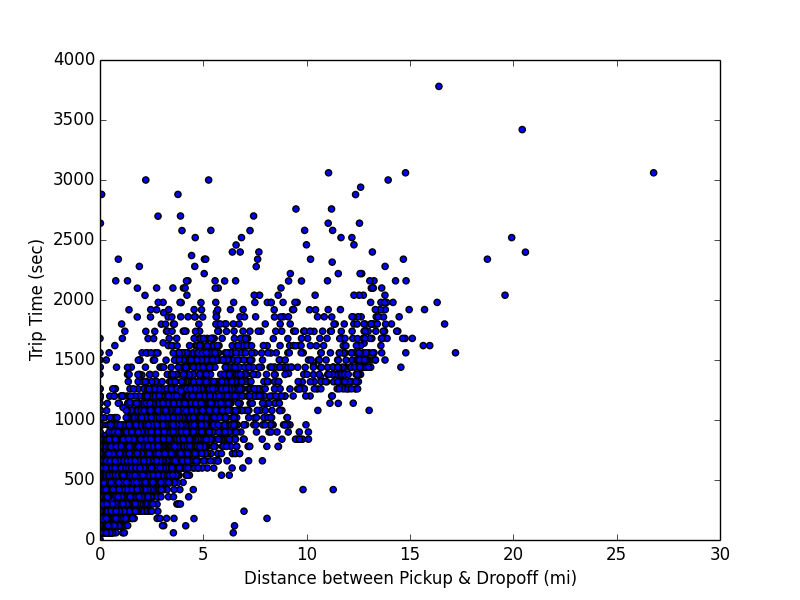
\includegraphics[scale=0.6]{3-mean.png}
  \caption{c - Distance btwn Pickup/Dropoff (mi) vs Trip Time (sec)}
  \end{figure}

  \item[d] The code used to separate training/test data is found in main.py. The code for calculating least squares fit (where w\textsubscript{0} represents the constant), OLS (sum of squared residuals), and TLS (sum of squared orthogonal distances) are all found in util.py [linReg, OLS, and TLS functions] and are called from the end of main.py. The results of the calculations are in table 2.

  \begin{center}
    \captionof{table}{d - LS Fit, OLS, TLS - Mean Filtering} 
    \begin{tabular}{| c | c |}
    \hline
    LS w\textsubscript{0} & 291.31518338 \\ \hline
    LS w\textsubscript{dist} & 97.15551468 \\ \hline
    OLS (test set) & 408074063.059 \\ \hline
    TLS (test set) & 43227.2961374 \\ \hline
    \end{tabular}
  \end{center}

  \item[e] As with part b, the new outlier filtering method is called in outlier.py [main, remove\_zeros, and median\_remove functions]. The new outlier removal approach is based on median absolute deviation (MAD) and is as follows:

    \begin{enumerate}
    \item[1] Remove any data points where trip time is 0
    \item[2] Remove any data points where the calculated distance between pickup and dropoff is greater than 3 MADs away from the median
    \end{enumerate}

  In this case, I treat MAD as the median absolute distance from the median of the observed calculated distance values. This filtering method removes a larger number of data points, down from 9882 to 9296. A MAD of 3 was chosen because it removed more points while maintaining the plot shape observed in part c. The new calculated values for least squares fit, OLS, and TLS are in table 3.

  \begin{center}
    \captionof{table}{e - LS Fit, OLS, TLS - Median Filtering} 
    \begin{tabular}{| c | c |}
    \hline
    LS w\textsubscript{0} & 217.19620176 \\ \hline
    LS w\textsubscript{dist} & 127.73425051 \\ \hline
    OLS (test set) & 278693727.935 \\ \hline
    TLS (test set) & 17079.9206978 \\ \hline
    \end{tabular}
  \end{center}

  The new outlier filtering method creates a lower OLS and TLS (which makes sense as the data is more clustered together) and a slightly lower correlation coefficient. Based on the metric of error (despite the higher CC), the results were slightly better. However, as this outlier filter doesn't filter on the dependent or independent variables we are modeling on, the difference appears to be minimal.

  Separately, as the MAD filtering resulted in a lower number of data points, I could see that sensible data representing longer taxi rides were eliminated (the maximum was reduce from 26 mi to 7 mi); therefore, it's possible this method may have over-removed outliers resulting in lower data quality. 

  \item[f] The new data is loaded from main.py where the script also reallocates training/testing data to match the new specifications. A new regression was ran with the new data sets an the results can be found in table 4. 

  \begin{center}
    \captionof{table}{f - LS Fit, Correlation Coefficient, OLS, TLS - trip\_data\_2} 
    \begin{tabular}{| c | c |}
    \hline
    LS w\textsubscript{0} & 291.9286576 \\ \hline
    LS w\textsubscript{dist} & 96.82391463 \\ \hline
    Correlation Coefficient (test set) & 0.773351576741\\ \hline
    OLS (test set) & 1.78226766223\e{12} \\ \hline
    TLS (test set) & 190090901.19 \\ \hline
    \end{tabular}
  \end{center}

  After incorporating a larger amount of data to create and test our linear model, the correlation coefficient has gone down as expected; however, the model still does a relatively good job representing the data. One thing to note is that the maximum distance for the test set is now 210 miles (compared to 26 for our test set). This may indicate that the outlier filtering method chosen was ineffective for larger quantities of data. 

  \item[g] One way to modify the parameter pickup time so that it's no longer cyclical is to use a binary value representing day and night. Based on our plots, it appears like there are distinct periods of time where there are higher and lower amounts of taxi traffic (in other words concentration of taxi use). By changing pickup time into a classification, we are better able to model and represent the clustering we are seeing in the plot. 

  This change is incorporated into the code with the change\_time and day\_night methods in the util file. The classifications we chose are 0-12 as one group and 12-24 as the other.

  \item[h] The new initial feature vector is built in retrieve.py. Normalization of data occurs in main.py following preprocessing through the normalize method of the util module. 

  The normalization method chosen for all the columns (except pickup time as it's now a binary classification value) is a normalization with respect to the sample mean and deviation. Specifically, the normalization formula used for trip distance is: 

  \begin{equation}
     nrm(dist)_i= \frac{dist_i - \overline{dist}}{\sigma_{dist}}
  \end{equation}

  \item[i] Once again, the testing and training data assignments had to be adjusted in main.py to match the new requirements. The regression results are detailed below in table 5.

  \begin{center}
    \captionof{table}{i - LS Fit, Correlation Coefficient, OLS, TLS - trip\_data\_1} 
    \begin{tabular}{| c | c |}
    \hline
    LS w\textsubscript{0} & 5.31335467\e2 \\ \hline
    LS w\textsubscript{dist} & 9.06941005\e1 \\ \hline
    LS w\textsubscript{pickup} & -3.06277802\e1 \\ \hline
    LS w\textsubscript{calcDist} & 4.09390616\e1 \\ \hline
    LS w\textsubscript{plong} & -4.67606828e\e{-1} \\ \hline
    LS w\textsubscript{plat} & 3.56264014 \\ \hline
    LS w\textsubscript{dlong} & 4.79637409\e{-1} \\ \hline
    LS w\textsubscript{dlat} & -5.36746377 \\ \hline
    Correlation Coefficient (test set) & 0.776974634364\\ \hline
    OLS (test set) & 1.39479790798\e{12} \\ \hline
    TLS (test set) & 6.57899357049\e{14} \\ \hline
    \end{tabular}
  \end{center}

  \item[j] Based on the results of our regression, the feature vector creates a more accurate linear model with a lower value for both error calculations (squared residuals and squared orthogonal distances) and a higher correlation coefficient. By providing additional features to train on, normalizing the data, and changing pickup time to a binary value, we were able to build a better model which captures more significant features than just travel distance. For example, based on our observations from part c, pickup time should have some effect on the observed travel time, and our new model actually would take this into account. Additionally, this model is trained on a significantly larger (and, hopefully, more representative) dataset, which should improve the quality of our model. 

  One potential concern is whether the features are all independent. For example, there should be some relationship between longitude, latitude, travel distance, and distance between pickup and dropoff.
\end{enumerate}

\section{The Titanic Disaster}

My first attempt at developing a model used what I'll call the `naive' set of features: age, sex, class, parch (parents/children) and sibsp (siblings). Fare was omitted as I assumed passenger class was already a good indicator for economic status and because some of the fares were extremely high and I was concerned about these outlier disproportionately affecting the model. I converted sex to a boolean (1 = male, 0 = female) and otherwise plugged everything directly into the training function. Because many ages were missing, I used sklearn.preprocessing's Imputer to replace unknown ages with the median value in both the training and testing phases. This model correctly predicted the survival of 77.033\% of passengers.\\

\noindent Unfortunately, this was as good as it got. I will discuss a sampling of my other models; I submitted ~20 to Kaggle. My first change was to use sklearn.preprocessing's `scale' method to normalize each feature so that it has zero mean and a standard deviation of 1.0. This did not in any way affect the accuracy of the model, leading me to believe that sklearn's LogisticRegression implementation already performs some scaling of the input features.\\

\noindent For the next iteration, I replaced `parch' and `sibsp' with a boolean feature called `has\_fam'. For each passenger, I summed the values of `parch' and `sibsp'. If the result was non-zero, has\_fam = True; otherwise, has\_fam = False. My reasoning was that people with many children (or children with more siblings) were no more likely to survive than someone with few children, and so large families might be skewing my results. However, this was not the case -- the accuracy of the model dropped slightly to 76.555\%.\\

\noindent I then tried excluding passengers with no age information from my training set. In general, the correlation coefficient for age was high, and I believed the use of the median in my training set might be skewing my model. Excluding these individuals reduced my training set from 891 to 714. For the test set, I continued to use the median for the age in incomplete records, as Kaggle requires a prediction for every person in the test set. Using the same features as the first attempt (age, sex, pclass, parch, and sibsp), but with the smaller training set, I got exactly the same result as the first attempt -- 77.033\%.\\

\noindent At this point, I was worried that my that something was wrong in my code, so I tried running the model using only one feature, age. Again excluding passengers with no age information from my training set, the accuracy was 62.679\%.\\

\noindent At this point I started trying every combination of features I could think of, without moving the result much off 76-77\%. I returned to my original set of features, but added fares, which actually reduced the accuracy to 76.555\%. Again believing that outlier prices could be skewing my results, I tried capping the fare. If the listed fare was \textgreater \$40, I set it equal to \$40 before training the model. This had no effect on the output -- the accuracy was still 76.555\%. Because fare correlates closely with passenger class, I was not particularly surprised that it didn't add much to my model.\\

\noindent I decided to try incorporating the cabin data, although it was extremely incomplete (less than half of the passengers in the training set have cabin data). I thought about trying to determine location on the ship from the cabin number, but couldn't find anything about the relationship between cabin number and location besides what letters corresponded to which passenger classes (which was already in the model). I tried using cabin as a boolean feature-setting it to True if the passenger had cabin data, False otherwise -- but again got an accuracy of 76.555\%.\\

\noindent At this point, I tried a more radical change by replacing every feature with a binary value, as follows:\\

\noindent Age: \textless 18 (child vs. adult)\\
\noindent Sex: Male\\
\noindent PClass: pclass != 3\\
\noindent parch: != 0\\
\noindent sibsp: != 0\\

\noindent For the binned input tests, I did not use fare or cabin. For the training data, I excluded entries with no age data. For the test data, I ran tests calling entries with no age data �`children' and `adults'. Regardless of how I categorized children, I got the same accuracy -- 76.555\%. I tried using only age, class, and sex, binned -- 76.555\%. I tried lowering the `child' threshold from 18 to 15 -- 76.555\%.\\

\noindent Finally, I tried mixing binary classifiers for some features while leaving others as continuous values. I tested binning age only (77.033\% -- back to original value) and age and class (77.033\% again).\\

\noindent I'm a little surprised at these results; I had thought my original, kitchen sink approach would be a starting point, and I would be able to get accuracy up by choosing my features more carefully and playing with the preprocessing algorithm, but this was not the case. In general, more information led to better results -- more features, more differentiation within the features. The only exceptions were fare, which did not improve the accuracy of the model, and cabin, which was sort of a shot in the dark to begin with. I'm looking forward to seeing if anyone in the class was able to crack 80\%.\\

\section{Written Exercise 1}
\begin{enumerate}
  \item[a] An example of a correlation coefficient (CC) value close to zero can be found in figure 4, a plot of Facebook friends against weekly granola bar purchases. A correlation coefficient of zero indicates that the data doesn't exhibit a linear relationship between the two variables.  In other words, any plot between two independent and unrelated variables should exhibit a CC close to zero. In this case, granola bars, as a relatively uncontroversial food (with people who both like and dislike them), should have a purchase rate that is unrelated to the number of Facebook friends they have and therefore a CC of 0. 

  \begin{figure}[H]
  \centering
  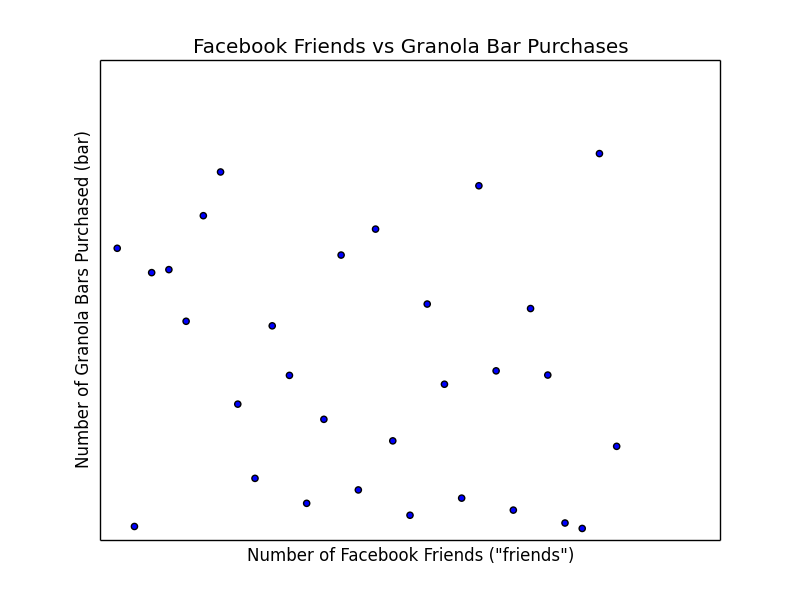
\includegraphics[scale=0.6]{Random.png}
  \caption{a - Correlation Coefficient of 0}
  \end{figure}

  \item[b] A correlation coefficient close to 1 indicates a strong positive linear relationship. In this case (Figure 5), a plot of vending machine revenue (at Cornell Tech) vs number of purchases was chosen. Because the vending machine (specifically the soda machine) only sells beverages at 75 and 125 cent price points, there will be a roughly linear relationship between number of purchases and total revenue earned (with noise incorporated because of the different prices). Because more purchases corresponds to more money made, a positive linear relationship is observed. 

  \begin{figure}[H]
  \centering
  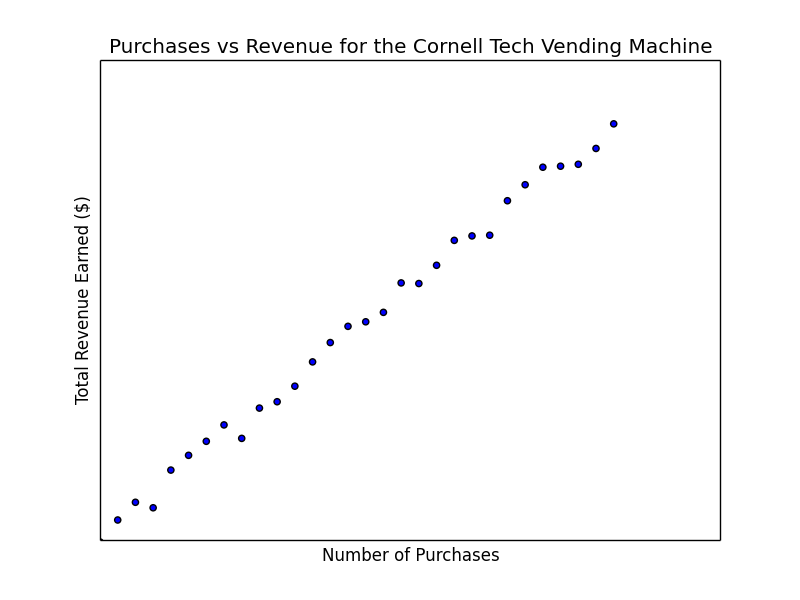
\includegraphics[scale=0.6]{Vending.png}
  \caption{b - Correlation Coefficient of 1}
  \end{figure}

  \item[c] A correlation coefficient close to -1 indicates a strong negative linear relationship. In this case (Figure 6), a plot of car velocity over time for a decelerating car was chosen. Because the car is breaking, it's speed drops which accounts for the negative relationship. Assuming a relatively constant rate of deceleration, the relationship between velocity and time is roughly linear with noise accounting for error margins in tools and the human limitations of maintaining a constant rate of deceleration while pressing a brake pedal. 

  \begin{figure}[H]
  \centering
  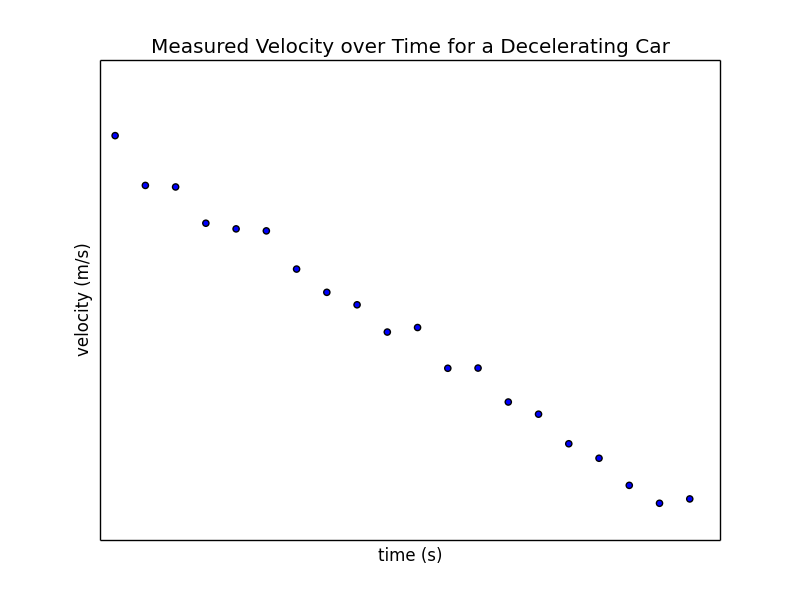
\includegraphics[scale=0.6]{Velocity.png}
  \caption{c - Correlation Coefficient of -1}
  \end{figure}
\end{enumerate}

\section{Written Exercise 2}
\begin{enumerate}
  \item[a] Here is such a graph (Figure 7), with the least-squares regression (applied to the training data) drawn in blue:

  \begin{figure}[H]
  \centering
  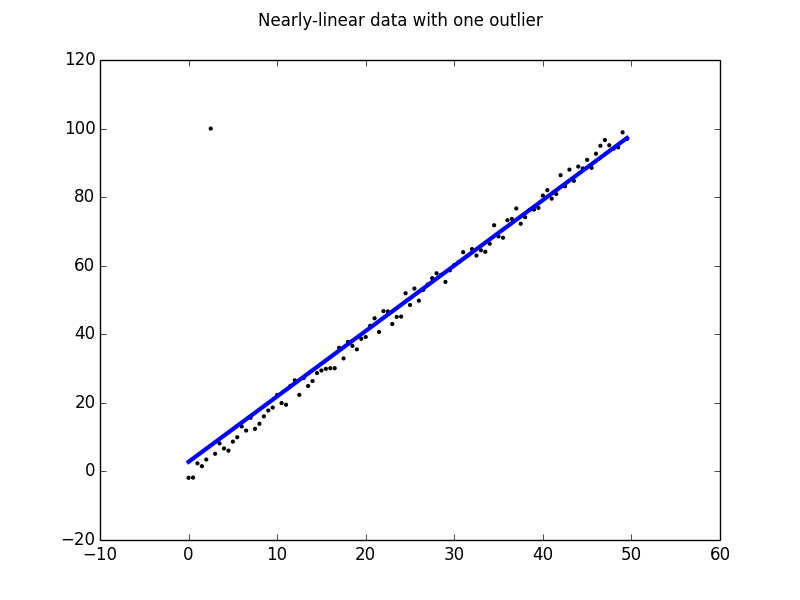
\includegraphics[scale=0.6]{leastsquaresoneoutlier.png}
  \caption{a - Nearly Linear Data with One Outlier}
  \end{figure}

  The data was generated by taking regularly-spaced x-values, calculating y = 2x, and adding a random number between -3 and +3 to each y. A single y-value was replaced with an outlier.

  As you can see, this outlier pulls the LSR considerably; the blue line is above most of the data on the left side and below the data on the right side. This is because the square of the residual is (obviously) much larger than the residual itself, so that outliers have a disproportionate weight in the error function. sklearn doesn't have an L1 regression (that I could find), so I didn't plot it here, but if I had calculated the regression based on minimizing the L1 norm the line would more closely fit my data, as the single outlier would not be weighted so heavily.

  \item[b] Here's (Figure 8) a dataset with multiple optimal solutions for L1-linear regression and only one for L2:

  \begin{figure}[H]
  \centering
  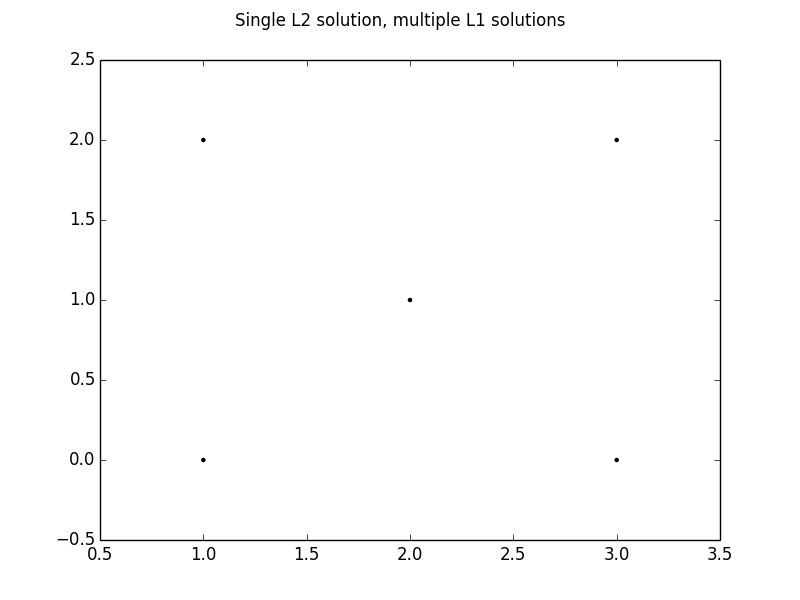
\includegraphics[scale=0.6]{q2partbnolines.png}
  \caption{b - Single L2 Solutions, One L1 Solution - no lines}
  \end{figure}

  There are infinite L1 solutions, but only one L2 solution. Here's (Figure 9) a plot with the L2 solution in blue and a pair of sample L1 solutions in red:

  \begin{figure}[H]
  \centering
  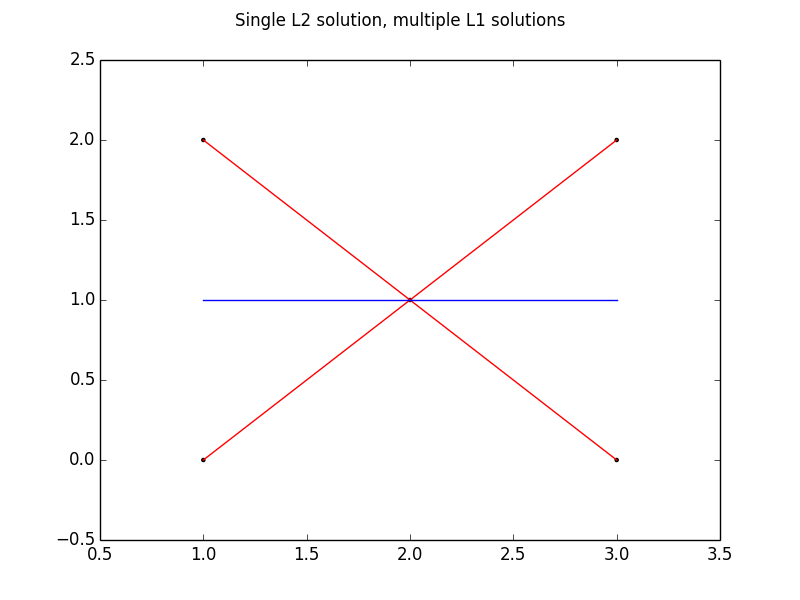
\includegraphics[scale=0.6]{q2partbwlines.png}
  \caption{b - Single L2 Solutions, One L1 Solution - with lines}
  \end{figure}

  There are only 5 points, so it's pretty easy to calculate out the residuals by hand. For the L1 solution with positive slope: \\

  Top left error: 2\\
  Bottom left: 0\\
  Center: 0\\
  Top right: 0\\
  Bottom right: -2\\
  
  Taking absolute values and summing, we get sum of absolute errors = 4. If you recalculate this for the red line with negative slope, you will get 4 again. Same with a horizontal line passing through the center point (the L2 solution). In fact, you will get the same answer for any line that passes between the outer pairs of points and through the center point. If you calculate the sum of the squares of the residuals for each line, though, you get: \\
  
  Positive slope: 2\textsuperscript{2} + 0 + 0 + 0 + (-2)\textsuperscript{2} = 8\\
  Negative slope: (-2)\textsuperscript{2}  + 0 + 0 + 0 + 2\textsuperscript{2}  = 8\\
  Horizontal: 1\textsuperscript{2}  + 1\textsuperscript{2}  + 0 + 1\textsuperscript{2}  + 1\textsuperscript{2}  = 4\\

  It's minimized for the horizontal line through the center. Obviously, this isn't very rigorous, but it's pretty clear that all plausible solutions to the L1 regression have the same sum-of-errors, while the L2 solution is unique.

  \item[c] Following on part (b), one crucial element is for the L1 norm minimization problem to be useful is to have a unique solution. Obviously the dataset I chose for part (b) is pretty artificial, but it would be tough to make predictions based on the L1 regression knowing that I could have chosen a solution with a positive, negative, or zero slope with equal justification. For pure convenience, you should also have a pretty good reason for rejecting the L2 norm (for example, avoiding the strong weighting of outliers discussed in part (a)), as it the existence of an analytical solution to the L2 problem makes it much easier to apply in practice.

\end{enumerate}
\end{document}
